Os materiais utilizados para o experimento foram: goniômetro, lâmpadas de diferentes elementos químicos, lupa e prisma de numeração 17.

para  o início da coleta de dados, o primeiro passo se resumiu a calibrar o goniômetro. Para tal, o prisma foi retirado do goniômetro, a luneta de leitura foi destravada e alinhada com com a entrada de luz da lâmpada de Sódio, travando a luneta. Na sequência, o foco da luneta foi ajustado de para que a cruz no interior da mesma pudesse ser visto de forma nítida, assim como a fenda de entrada de luz; o parafuso de ajuste fino foi empregado para garantir que a cruz se alinhasse com o lado fixo da fenda. Para finalizar o ajuste, o disco graduado do goniômetro foi liberado seu "zero" foi alinhado com o "zero" da luneta.

Para próxima etapa do experimento, foi preciso determinar o ângulo $\alpha$ do ápice do prisma, isto é, a separação angular entre as duas faces do prisma mais próximas à fonte de luz. Para isto, considerou-se os dois raios luz $L_1$ e $L_2$ refletidos pelas faces do prisma, e o resultado geométrico que mostra que $\Delta \theta_L = 2\alpha$, ou seja, a separação angular entre os raios é igual ao dobro do ápice, como ilustrado abaixo.

\begin{figure}[H]
	\centering	    
	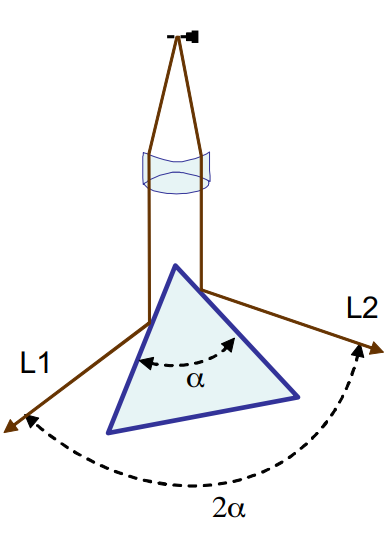
\includegraphics[scale=0.35]{figuras/alpha.png}
	\caption{Diagrama para a obtenção de $\alpha$}
	\label{fig:alpha}
\end{figure}

Com o ápice do prisma devidamente determinado, a fim de determinar o coeficientes A e B da equação de Cauchy $n(\lambda) = A + \frac{B}{\lambda^2}$, mostrou-se necessário coletar dados para o ângulo de desvio mínimo $\delta_{min}$ das raias espectrais de dispersão e determinar o índice de refração através da relação:

\begin{equation}
    n(\delta_{min}) = \frac{\sin(\frac{\alpha + \delta_{min}}{2})}{\sin(\frac{\alpha}{2})}
    \label{eqn1}
\end{equation}

 Assim, possibilitando a construção de um gráfico de $n$ por $1/\lambda^2$ em que A e B equivalem, respectivamente, aos coeficientes linear e angular do ajuste.

Para determinação dos desvios mínimos de cada raia espectral, lâmpadas baseadas em diferentes elementos químicos foram empregadas, no caso, os elementos utilizados foram: Sódio, Mercúrio, Cádmio e Hélio. O procedimento experimental consistia da observação das raias espectrais mais intensas geradas a partir da luz emitida pelas lâmpadas, de forma que o ângulo mínimo de dispersão de cada uma delas fosse medido com auxilio do goniômetro. Na sequência, os comprimentos de onda de cada raia foi obtido a partir de valores tabelados na literatura. Foram coletados dados para as 3 raias mais intensas de cada lâmpada, com exceção do Hélio, em que 4 raias puderam ser observadas com clareza.

Por fim, com os dados coletados, foi possível determinar os coeficiente A e B e por fim, utilizando a equação \ref{eqn1} e seguinte inversão da equação de Cauchy:
\begin{equation}
    \lambda = \sqrt{\frac{B}{n(\delta_{min})-A}}
\end{equation}
foi gerada um curva que pode ser empregada como espectrômetro.



